\section{Background}

--- The maturation of the Web platform has given rise to sophis- ticated and demanding Web applications such as interactive 3D visualization, audio and video software, and games. With that, efficiency and security of code on the Web has become more important than ever. Yet JavaScript as the only built- in language of the Web is not well-equipped to meet these requirements, especially as a compilation target.



\subsection*{Web technologies}

The development of the world wide web has provided HTML, CSS, and JavaScript.

\subsection{JavaScript}

JavaScript was introduced 1995 with the intention to solve small tasks, e.g. validation of input data and small animations \parencite{Moller2018}. The last few years the web has evolved from simply being a platform for websites to also be a platform for (webb-)applications/apps.

JavaScript was a major addition to the set of web technologies. It is estimated that X \hl{add numbers with references here} use JavaScript.

[...]

\begin{figure}[!h]
\centering
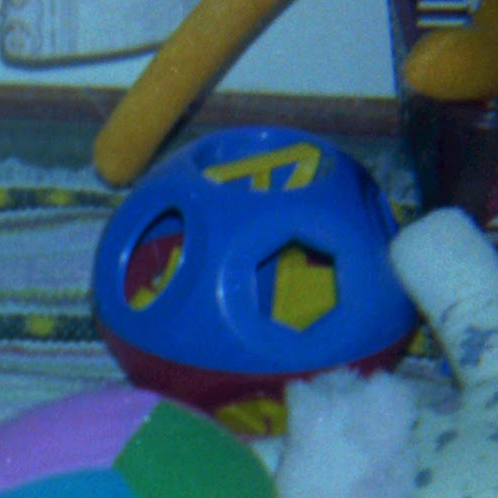
\includegraphics[width=6.5cm,height=6.5cm,keepaspectratio]{toy}
\caption{My personal plastic sphere of differently shaped holes.}
\label{toy}
\end{figure}


\begin{table*}\centering
\ra{1.3}
\begin{tabular}{@{}rrrrcrrrcrrr@{}}\toprule
& \multicolumn{3}{c}{$w = 8$} & \phantom{abc}& \multicolumn{3}{c}{$w = 16$} &
\phantom{abc} & \multicolumn{3}{c}{$w = 32$}\\
\cmidrule{2-4} \cmidrule{6-8} \cmidrule{10-12}
& $t=0$ & $t=1$ & $t=2$ && $t=0$ & $t=1$ & $t=2$ && $t=0$ & $t=1$ & $t=2$\\ \midrule
$dir=1$\\
$c$ & 0.0790 & 0.1692 & 0.2945 && 0.3670 & 0.7187 & 3.1815 && -1.0032 & -1.7104 & -21.7969\\
$c$ & -0.8651& 50.0476& 5.9384&& -9.0714& 297.0923& 46.2143&& 4.3590& 34.5809& 76.9167\\
$c$ & 124.2756& -50.9612& -14.2721&& 128.2265& -630.5455& -381.0930&& -121.0518& -137.1210& -220.2500\\
$dir=0$\\
$c$ & 0.0357& 1.2473& 0.2119&& 0.3593& -0.2755& 2.1764&& -1.2998& -3.8202& -1.2784\\
$c$ & -17.9048& -37.1111& 8.8591&& -30.7381& -9.5952& -3.0000&& -11.1631& -5.7108& -15.6728\\
$c$ & 105.5518& 232.1160& -94.7351&& 100.2497& 141.2778& -259.7326&& 52.5745& 10.1098& -140.2130\\
\bottomrule
\end{tabular}
\caption{Caption}
\end{table*}

The table \ref{table:one} is an example of referenced \LaTeX elements.
\begin{table}[h!]
\centering
\begin{tabular}{@{}llll@{}} 
\hline
 Col1 & Col2 & Col2 & Col3 \\ [0.5ex] 
 \hline
 1 & 6 & 87837 & 787 \\ 
 2 & 7 & 78 & 5415 \\
 3 & 545 & 778 & 7507 \\
 4 & 545 & 18744 & 7560 \\
 5 & 88 & 788 & 6344 \\ [1ex] 
 \hline
\end{tabular}
\caption{Table to test captions and labels}
\label{table:one}
\end{table}

\clearpage

\begin{lstlisting}[label=lst1,language=JavaScript,numbers=none,caption=prototype.js,frame=shadowbox]
Name.prototype = {
    methodName: function(params){
        var doubleQuoteString = "some text";
        var singleQuoteString = 'some more text';
        // this is a comment
        if(this.confirmed != null && typeof(this.confirmed) == Boolean && this.confirmed == true){
        document.createElement('h3');
        $('#system').append("This looks great");
        return false;
        } else {
        throw new Error;
        }
    }
}
\end{lstlisting}

\blindtext\\
Listing \ref{lst1}

\begin{lstlisting}[language=JavaScript,numbers=none,caption=Listing 2,frame=shadowbox]
function isPrime(value) {
    for(var i = 2; i < value; i++) {k
        if(value % i === 0) {
            return false;
        }
    }
    return value > 1;
}
\end{lstlisting}

\blindtext

\subsubsection{Optimizing/ations}

[...]

A major problem with optimizing is that fact that JavaScript is a loosely typed language, which means that the interpreter needs to be able to store any type of data in any variable. If the interpreter instead would be able to distinguish between which type of data each variable can store, it would be much easier to optimize.

\subsubsection{JIT}

The manufacturers of web browsers has in the last few years focused on optimizing JavaScript performance in different ways, such as introducing ''Just-In-Time'' (JIT) compilers \parencite{HerreraChenLavoieHendren2018}.

\subsubsection{AOT}



\subsubsection{TypeScript}

TypeScript \hl{REF} is a superset of JavaScript that adds type information. Type information allows the programmer to see mistakes sooner during the development phase rather than later in runtime.

\begin{verbatim}
$ cat > prime.ts
function isPrime(value: number) {
    for(var i = 2; i < value; i++) {
        if(value % i === 0) {
            return false;
        }
    }
    return value > 1;
}
\end{verbatim}

This does not directly solve the problem, but decreases the number of runtime errors, and enables future backend optimizations such as improved guesses by the JIT-compiler.

\subsubsection{ASM.js}

ASM.js is a subset of JavaScript that is known to be heavily optimized.

There are transpilers between JavaScript and ASM.js such as EmScripten.

\begin{verbatim}
function strlen(ptr) { // calculate length of C string
    ptr = ptr|0;
    var curr = 0;
    curr = ptr;
    while (MEM8[curr]|0 != 0) {
        curr = (curr + 1)|0;
    }
    return (curr - ptr)|0;
}
    
\end{verbatim}

\paragraph{x}

x

\subparagraph{y}

y

\subsection*{Web applications}

Web applications are made possible through use of JavaScript.

However according to \textcite{ReiserBlaser2017} there is always a desire for higher performance. \textcite{Zakai2018} describes JavaScript as an obstacle for demanding/truly high-performing applications/apps.

Web applications can be executed on the server with a thin wrapper in the client, in the client with our without a server counterpart. Or, as a combination of both client and server computation.

\subsubsection{Server}

[...]

\subsubsection{Client}

[...]

\subsection{WebAssembly}

WebAssembly\footnote{https://webassembly.org/} (Wasm) is by definition according to \textcite{HaasRossbergSchuffTitzerHolmanGohmanWagnerZakaiBastien2017} a portable assembly-language for web browsers and future adaptations. Technically WebAssembly is bytecode created by \emph{compiling} (any form of) code to WebAssembly \parencite{Watt2018} which then can be executed in any WebAssembly-engine. This can be compared with JavaScript-code that is \emph{interpreted} while running inside a JavaScript-engine.

WebAssembly can be seen as a successor to earlier technologies such as asm.js from Mozilla and Native Client (NaCL) from Google. NaCL executes native code in a separate part of Chrome and asm.js  \parencite{Zakai2018} is a subset of JavaScript optimized for performance \parencite{VanEsNicolayStievenartDHondtDeRoover2016} and can be interpreted in any web browser.

Earlier work on what today is WebAssembly has also resulted in EmScripten \parencite{Zakai2011}, a compiler based on LLVM \parencite{LattnerAdve2014} that originates as a transpiler from JavaScript to asm.js \parencite{Zakai2011} that has been further developed \parencite{HaasRossbergSchuffTitzerHolmanGohmanWagnerZakaiBastien2017} and is now able to compile both JavaScript and C/C++ to both asm.js and WebAssembly. EmScripten is the most common compiler to compile WebAssembly.

WebAssembly is the result of joint research and development between Apple, Google, Microsoft and Mozilla \parencite{HaasRossbergSchuffTitzerHolmanGohmanWagnerZakaiBastien2017}. WebAssembly has as the first technology since JavaScript \emph{full} support in Chrome, Edge, Firefox and Safari \parencite{Moller2018}. Those web browsers that does not support WebAssembly can according to \textcite{HaasRossbergSchuffTitzerHolmanGohmanWagnerZakaiBastien2017} use asm.js as ''polyfill''. WebAssembly is already being used where performance is of high importance, such as to generate cryptocurrency \parencite{RuthZimmermannWolsingHohlfeld2018}.

Initially WebAssembly supports code written in C/C++ \parencite{HaasRossbergSchuffTitzerHolmanGohmanWagnerZakaiBastien2017}. 
The focus on C/C++ is largely based on WebAssembly implementation limitations such as the lack of garbage collection. According to \textcite{HaasRossbergSchuffTitzerHolmanGohmanWagnerZakaiBastien2017} its a highly prioritized goal to allow WebAssembly to gain to access the web browsers built in garbage collector and that way support languages that use garbage collection.

WebAssembly is loaded as a module via a JavaScript API or another WebAssembly module \parencite{HaasRossbergSchuffTitzerHolmanGohmanWagnerZakaiBastien2017}. According to \textcite{Moller2018} it's \emph{not} a goal to have WebAssembly replace JavaScript, the idea is that they \emph{complement} each other. One example of how JavaScript and WebAssembly could complement each other is to replace large portions of JavaScript within popular JavaScript-frameworks with WebAssembly, but keep the JavaScript API towards the developer and thus only provide the benefit of performance.

WebAssembly is new technology. The first articles about WebAssembly was published in 2017 \parencite{HaasRossbergSchuffTitzerHolmanGohmanWagnerZakaiBastien2017,ReiserBlaser2017}.

\subsection{Benchmarking}

\parencite{LehmannPradel2018,MalleGiulianiKiesebergHolzinger2018}

[...]

WebAssembly is according to \textcite{HaasRossbergSchuffTitzerHolmanGohmanWagnerZakaiBastien2017} an option to JavaScript with higher performance. Higher performance makes way for demanding/truly high-performing applications/apps.
